%index
\chapter{Introducci\'on}
Durante los a\~nos 1990 a 2016, la Organizaci\'on mundial de la salud ha recopilado datos sobre los distintos riesgos met\'abolicos que han afectado a distintos pa\'ises, lo cual ha encontrado que alrededor de 1.6 millones de personas, mueren anualmente por no realizar la suficiente actividad f\'isica. Por lo tanto, la inactividad f\'isica es un problema mundial que afecta hoy en d\'ia y principalmente en Guatemala, ya que en el a\~no 2006, se realiz\'o una encuesta de enfermedades no transmisibles en la comunidad de Villa Nueva, Guatemala. La cual concluyeron que alrededor de 27.68\% de los guatemaltecos, presenta sedentarismo por no realizar ninguna actividad f\'isica.
\medbreak
Debido a este problema, la Organizaci\'on de las Naciones Unidas ha creado 17 objetivos para el desarrollo sostenible del planeta, en donde el tercer objetivo se relaciona con la salud y bienestar de la personas, la cual busca reducir las muertes prematuras por enfermedades no transmisible, a partir de la nuevas tecnolog\'ias y educaci\'on. Por lo tanto, la Organizaci\'on mundial de la salud impulsa el movimiento: "Por tu salud, muev\'ete", y a ra\'iz de esto, en el a\~no 2018, el ministerio de salud p\'ublica y asistencia social de Guatemala impulsa el lema "Salud para todos y todas, en todas partes".
\medbreak
Partiendo de este lema, se ha creado este proyecto de ingenier\'ia, la cual con la ayuda de la interfaz de programaci\'on de aplicaciones y el kit de desarrollo de software del dispositivo Kinect, se crear\'a un modelo de reconocimiento de movimiento por cada deporte seleccionado. No obstante, cada modelo ser\'a comparado por otros dos modelos, que ser\'an entrenado por el mismo algoritmo, pero con distintos datos de entrenamiento y testeo, con la finalidad de encontrar el error promedio del modelo principal. 
\medbreak
Por otra parte, el modelo de reconocimiento de movimiento ser\'a utilizado para el conteo de repeticiones de un Tabata, entrenamiento deportivo de alta intensidad, que produce y consume la energ\'ia necesar\'ia para realizar actividad f\'isica.
\medbreak
En definitiva, esta investigaci\'on es importante debido que aportar\'a a los proyectos guatemaltecos de visi\'on artificial y as\'i mismo motivar\'a a las personas a realizar actividad f\'isica a partir de los resultados proporcionado en un rutina Tabata.
\newpage 
\section{Lo escrito sobre el tema} \label{tr}
\subsection{Sistema de detecci\'on y reconocimiento de la postura corporal basado en Kinect} \label{tr:1}
\citeA{pisharady2013kinect} mencionan que alrededor del 66\% de la poblaci\'on mundial  utilizan la comunicaci\'on no verbal, dicha comunicaci\'on esta conformado por posturas corporales, gestos, expresiones faciales y movimientos corporales. Por lo tanto, los autores propone un sistema para detectar expresiones est\'aticas -i.e. Posiciones que no cambian durante un per\'iodo de expresi\'on-.
\medbreak
Dicho sistema detecta y reconoce posturas corporales de una persona con la ayuda del sensor del Kinect, ya que le proporciona la posici\'on de las articulaciones del cuerpo humano -e.g. mano, codo, hombro, rodilla- en un espacio vectorial definido por el sensor. Posteriormente se calcula las caracter\'isticas angulares respecto a dos vectores de articulaciones, por ejemplo; para encontrar la caracter\'istica angular del codo derecho se utiliza los vectores de la mano derecha y hombro derecho.
\medbreak
Por otro lado, \citeA{pisharady2013kinect} analizaron un total de 11 componentes angulares para entrenar una \acrfull{SVM} de n\'ucleo polin\'omico, con la finalidad de detectar un total de 10 movimientos est\'aticos -e.g. Pararse, agacharse, hablar por tel\'efono-, as\'i mismo el entrenamiento consisti\'o en tomar 6000 muestras de posturas de 6 personas diferentes -i.e. Cada persona realiz\'o 100 muestras por postura-.
\medbreak
Finalmente, \citeA{pisharady2013kinect} recolectaron un total de 5000 muestras positivas (correspondiente a los 10 movimientos est\'aticos).  Como resultados obtuvieron una falla de pron\'ostico de 1.46\%, debido que el sensor Kinect no podr\'ia rastrear correctamente el seguimiento esqueleto.
\subsection{Reconstruci\'on de posturas en tiempo real} \label{tr:2}
\citeA{shum2013real} determinaron que el sensor Kinect tiene un problema con el reconocimiento de postura a la hora de interactuar con objetos externos -e.g. Baloncesto, levantamiento pesas-, por lo tanto, algunos datos de seguimiento de esqueleto son incorrecto, de tal manera que lo autores propone un m\'etodo para medir la confiabilidad de datos al momento de detectar una postura.
\medbreak
Para determinar el nivel de confiabilidad de datos, \citeA{shum2013real}, contruyeron una base de datos de 21590 posturas est\'aticas, la cual mide los \'angulos entre articulaciones. Esto permite  extraer las 30 posturas que se asemeja al movimiento real -i.e. 30 vecinos m\'as cercanos-.  Posteriormente, localizan cada postura en un nuevo espacio vectorial -i.e Espacio diferente al Kinect-, seleccionando as\'i la postura que tenga la menor distancia entre los puntos vectoriales.
\medbreak
Finalmente, \citeA{shum2013real}, realizaron las pruebas a 27 personas, dichas pruebas consist\'ia en hacer actividades con objetos externos -e.g. caja, silla, l\'apiz, pelota-, analizando la parte superior (Arriba de las caderas) e inferior de cada persona. Como resultados a estas pruebas, encontraron una diferencia de distancia de 9 a 13 cm entre la postura real y de referencia, determinando as\'i un nivel de confiabilidad del de 80\% respecto a dos sistemas de detecci\'on de movimiento en tiempo real \cite{shum2011fast,shum2012real}.
\subsection{Detecci\'on de posturas a la hora de sentarse para prevenir el s\'indrome de los trabajadores de oficina usando el Kinect} \label{tr:3}
\citeA{paliyawan2014prolonged} estudiaron el s\'indrome del trabajador de oficina, la cual consiste en un grupo de s\'intomas que tiene los trabajadores por los h\'abitos no saludables -e.g. La postura a la hora de sentarse-, provocando en la persona distintos dolores corporales.
\medbreak
En relaci\'on a los riesgos de salud de una persona, \citeA{paliyawan2014prolonged}, investigaron que una de las causas de una enfermedad no transmisible es debido al tiempo prolongado de estar sentado, sin realizar ning\'una actividad f\'isica. Por lo tanto, los autores  proponen un sistema que detecta las posturas a la hora que esta trabajando en una oficina.
\medbreak
Para realizar dicho sistema, \citeA{paliyawan2014prolonged} estudiaron las posturas de 28 personas,  recolectaron un total de 1326 posturas. De igual manera, cada postura conten\'ia un total 31 atributos -i.e. Tiempo y posici\'on de 10 articulaciones-. Posteriormente, el sistema procesa los datos y encuentra la \gls{diseuc} entre los datos consecutivos, permitiendo normalizar las distancias m\'aximas y m\'inimas por persona y en forma general -i.e. Conjunto de personas analizadas-.
\medbreak
Finalmente, el sistema detecta una buena o mala posici\'on, a partir de cuatros m\'etodos de clasificaci\'on: \gls{arbdec}, \gls{redneu}, \gls{bayesian} y 5 vecinos m\'as cercanos. Por lo tanto, para seleccionar el mejor m\'etodo, los autores realizaron una prueba a 10 personas, de tal manera que el mejor  clasificador es de \acrfull{KNN}, debido que tuvo una precisi\'on de  98.83\%. 
\subsection{Comparaci\'on de los m\'etodos de machine learning para el prop\'osito de la detecci\'on de la ca\'ida humana} \label{tr:4}
\citeA{stremy2014comparison}, estudian sobre la  ca\'ida en persona mayores, la cual determinaron que la ca\'ida  es el accidente m\'as peligros y frecuente que puede sufrir un anciano, debido que las personas de tercera edad se cae al menos una vez al a\~no y es la causa principal de muerte accidental en personas mayores de 65 a\~nos. Por lo tanto, los autores proponen un sistema que permite monitorear a los humanos y detectar posibles ca\'idas.
\medbreak
En relaci\'on a los datos del entrenamiento del sistema, los autores recolectaron un total de 450 actividades, realizada por 5 personas. As\'i mismo, clasificaron las actividades en tres movimientos est\'aticos: Parado, sentado y acostado. En cada movimiento est\'atico, obtiene la posici\'on de 20 articulaciones del cuerpo -e.g. Mano, codo, hombro-. Luego normaliza los datos a partir de la distancia desde el piso -i.e. Recta entre las articulaciones del p\'ie- a cada punto de articulaci\'on, con el fin objetivo de entrenar tres m\'etodos de clasificaci\'on: \gls{svmia}, \gls{bayesian} y \gls{arbdec}.
\medbreak
Para seleccionar el algoritmo clasificador, los autores realizaron 120 pruebas -i.e. 40 pruebas por cada movimiento est\'aticos-, en donde determinaron  que el \gls{arbdec} es la mejor opci\'on para ese proyecto, debido que tiene una exactitud de 93.3\% para detectar ca\'idas.
\subsection{Sistema de monitoreo de sue\~no usando el sensor Kinect} \label{tr:5}
\citeA{lee2015sleep} indican que hoy en d\'ia, la vida humana est\'a intensamente ocupada debido al constante trabajo y actividad, provocando en las personas el insomnio -i.e. Perdida del sue\~no-. As\'i mismo, el insomnio es conocido por discapacidades de aprendizaje y procesos ineficiente de trabajo. Por lo tanto, los autores presenta un sistema que recopila el movimiento y la postura durante el sue\~no.
\medbreak
Para calcular el movimiento de sue\~no, los autores tomaron la posici\'on de 19 articulaciones por cada medio segundo, posteriormente, el sistema calcula la \gls{diseuc} respecto a la posici\'on actual y anterior. Luego, suma todas las distancias de articulaciones para encontrar la distancia total y finalmente normaliza los datos, sumando todos los valores del movimiento respecto a una hora.
\medbreak
En relaci\'on en la detecci\'on de posturas, \citeA{lee2015sleep} separan el plano cartesiano en 6 cuadrantes, respecto a 3 l\'ineas gu\'ias: Linea media (articulaciones del Cuello y base de la columna vertebral), linea superior (Linea perpendicular a la articulaci\'on superior  de la columna vertebral) y la linea inferior (Linea perpendicular a la articulaci\'on base  de la columna vertebral). Posteriormente, localiza el cuadrante de las articulaciones de las manos y rodillas respecto a su ubicaci\'on, con el fin de objetivo de detectar 5 posiciones de sue\~no.
\medbreak
Finalmente para realizar las pruebas del sistema, reunieron a 20 estudiantes, en donde realizaron un monitoreo del sue\~no alrededor de 7 horas. La cual concluyeron que la perdida del sue\~no influye en el movimiento, debido que algunos estudiantes durmieron mal, ya que permanecieron en constante movimiento (Alrededor del 60 \% del  movimiento de sue\~no),
\subsection{Entrenador personal virtual a tr\'aves del sensor de Kinect} \label{tr:6}
\citeA{jin2015virtual} mencionan que el ejercicio es una de las actividades que se han pr\'acticado durante mucho tiempo, sin embargo, se ha ignorado debido al alto costo y el tiempo que se requiere -e.g. Ir al gimnasio-, adem\'as las aplicaciones o productos deportivos solo proporciona una gu\'ia deportiva y no existe una interacci\'on con los atletas. Por lo tanto los autores proporciona un entrenador virtual que brinda una gu\'ia de entrenamiento y una evaluaci\'on en tiempo real durante la actividad f\'isica de los usuarios.
\medbreak
La gu\'ia de entrenamiento consiste en una base de datos que identifica las acciones est\'aticas. Cada acci\'on es analizada como un modelo discreto de la aplicaci\'on, Visual Gesture Builder, posteriormente analiza la trayector\'ia  respecto a dos movimientos est\'aticas, en donde calcula las distancias euclidianas en relaci\'on a la posici\'on actual y anterior -i.e. Frame capturado un segundo antes- por cada articulaci\'on del cuerpo.
\medbreak 
Posteriormente realizan una evaluaci\'on de tiempo real por medio del puntaje de salud, dicho puntaje consiste en asignar un peso y calcular la distancia de cada articulaci\'on del cuerpo en relaci\'on a la posici\'on real y la posici\'on gu\'ia -i.e. Movimiento est\'atico-.
\medbreak 
Finalmente para entrenar el sistema, \citeA{jin2015virtual} recopilan v\'ideos por cada movimiento de an\'alisis, recolectando una muestra  de movimientos realizadas por un profesional o atleta.
\subsection{Una comparaci\'on entre las t\'ecnicas heur\'isticas y de aprendizaje autom\'atico en la detecci\'on de ca\'idas con Kinect v2} \label{tr:7}
En la publicaci\'on, A Comparison Between Heuristic And Machine Learning Techniques In Fall Detection Using Kinect v2 \cite{amini2016comparison}, se compara 2 m\'etodos para detectar la posici\'on, velocidad y aceleraci\'on de un usuario al momento de que un usuario sufre de una ca\'ida.
\medbreak 
Seg\'un \citeA{amini2016comparison}, el primer m\'etodo se basa en la \gls{Heur} que aprovecha la funcionalidad del seguimiento de esqueleto, la cual consiste en analizar la distancia entre la articulaci\'on de la cabeza y el suelo -i.e. Recta respecto a las articulaciones de los p\'ies-, mientras que el segundo m\'etodo consiste en una m\'aquina de aprendizaje, usando la funcionalidad visual y constructor de gestos -i.e. Visual Gesture Builder del sensor Kinect-, la cual analiza el escenario y le asigna un color a las posibles fallas de ca\'idas.
\medbreak 
As\'i mismo, \citeA{amini2016comparison} mencionan que para el primer m\'etodo los datos se fueron determinando a partir de la ecuaci\'on escalar de un plano, mientras que en el segundo m\'etodo se utiliz\'o el algoritmo AdaBoostTrigger -i.e Modelo discreto de Visual Gesture Builder-.
\medbreak 
Finalmente, \citeA{amini2016comparison} realizaron una prueba con 11 personas, la cual concluyeron que para el primer m\'etodo detectaba un 95.42\% de las ca\'idas, mientras que para el segundo m\'etodo fue de 88.33\%, por lo tanto seleccionaron el primer modelo.
\subsection{Sistema de detecci\'on de posiciones de un humano en tiempo real} \label{tr:8} 
En la publicaci\'on, Machine learning for real time poses classification using Kinect skeleton data \cite{choubik2016machine}, habla sobre el desarrollo de un sistema que reconoce 18 posiciones distintas del ser humano.
\medbreak 
Para construir el sistema,  \citeA{choubik2016machine} comparan cuatros modelos matem\'aticos: El primer modelo consist\'ia en una \gls{svmia} que consiste en encontrar un margen \'optimo dentro del espacio vectorial, con la finalidad de separar correctamente los datos. Dicho modelo se compara tres funciones del Kernel: Lineal, Polinomial y de \gls{brad} (RBF). As\'i mismo, el segundo modelo matem\'atico era una \gls{redneu} de dos funciones distintas: \gls{sigm}  y \gls{gaus}. De igual manera, el tercer modelo consiste en implementar el modelo \gls{knnia}, que determina la distancia de cada punto vectorial con su respectiva etiqueta y se ajusta un valor K, seg\'un el entrenamiento de datos. Finalmente el cuarto modelo consist\'ia en un , \gls{bayesian} la cual pronostica la posici\'on dado el punto vectorial.
\medbreak 
Igualmente, \citeA{choubik2016machine} entrenaron el sistema con 1800 datos, por cada dato se determin\'o  20 distancias relativa entre dos puntos de articulaci\'on -e.g. la altura entre codo derecho y hombro derecho-.
\medbreak 
Como resultados de las pruebas,  \citeA{choubik2016machine} seleccionaron el algoritmo lineal-SVM, debido que tiene un 99.05\% de precisi\'on.
\subsection{Sistema que detecta pasos de bailes k-pop} \label{tr:9} 
En la publicaci\'on, Classification of K-Pop Dance Movements Based on Skeleton Information Obtained by a Kinect Sensor \cite{kim2017classification}, habla sobre el Desarrollo de un sistema que reconoce 800 movimientos de baile de K-Pop.
\medbreak 
En relaci\'on al reconocimiento de bailes, el sistema identifica los 6 principales \'angulos de movimiento del cuerpo -i.e. Componente principal para el an\'alisis-, posteriormente determina la \gls{matcov}, la cual determina el valor de variaci\'on respecto a cada componente de an\'alisis,  esto permite obtener un an\'alisis discriminante lineal -i.e. Que tan dispersos se encuentra los valores-.
\medbreak 
Luego ingresa los datos de dispersi\'on para entrenar una  \acrfull{ELM}, y obtener una mayor exactitud en las respuesta en tiempo real.
\medbreak 
Finalmente, \citeA{kim2017classification} recolectaron un total de 1656 datos de entrenamiento por cada movimiento de baile, dichos datos fueron utilizado para entrenar tres modelos matem\'aticos: el primer modelo consist\'ia en un KNN, la cual reconoc\'ia entre 88\% a 92\% de los pasos de baile. El segundo modelo consist\'ia en un SVM, la cual detectaba entre 62\% a 84\% de los pasos de baile y finalmente el tercer modelo consist\'ia en una \gls{elmia}, la cual reconoc\'ia entre 75\% a 95\% de los bailes.
\medbreak 
Por lo cual, \citeA{kim2017classification}  seleccionaron el modelo ELM, debido que el modelo reconoce un porcentaje mayor de pasos de baile, as\'i mismo indica que el \'exito de reconocimiento de baile es debido la extracci\'on principal de componentes de datos -i.e. \'Angulos de cuerpo-, la reducci\'on de los datos y finalmente  el dise\~no clasificador.
\subsection{Comparaci\'on de trabajos relacionados} \label{tr:10}
Tal como se muestra en la tabla de la siguiente p\'agina, el sensor Kinect se ha utilizado para controlar algunos problemas de salud, a partir de distintos m\'etodos de clasificaci\'on entrenados por  movimientos est\'aticos. -e.g. \'Arboles de decisiones, KNN, Adaptive Boosting-. Por lo tanto para el presente proyecto, el movimiento flu\'ido se analiza por varios movimientos est\'aticos -i.e. Pasos del movimiento-, la cual se etiqueta con un valor decimal establecido por el modelo Random Forest Regresssion de Visual gesture Builder, de modo que se obtenga un factor de movimiento -i.e. Valor n\'umerico que representa la transici\'on que tiene el movimiento-. As\'i mismo se utiliza este modelo de clasificaci\'on debido que toma en consideraci\'on distintas variables del movimiento cinem\'aticos -e.g. Posici\'on, velocidad, desplazamiento, \'angulos de movimiento, Fuerza, torque muscular-, que son capturados por medio de v\'ideos de rutinas deportivas -i.e. Atletas que realizan series de repeticiones del movimiento-.
\medbreak
Igualmente los trabajos relacionados tiene en com\'un el proceso de la recolecci\'on de los datos, debido que selecciona articulaciones de estudio, lo cual para el presente proyecto se elige la articulaci\'on de an\'alisis, cuya funci\'on es medir la distancia de profundidad adecuada para ejecutar correctamente el seguimiento de esqueleto, adem\'as del conjunto de articulaciones que interviene para realizar un movimiento.
\medbreak
Por otro lado, este trabajo de investigaci\'on es distinto a los otros trabajos relacionados, debido que es un proyecto que se enfoca a verificar si una persona esta movi\'endose para satisfacer la actividad f\'isica necesaria por medio de repeticiones de un movimiento deportivo -e.g. Saltos, patadas, sentadillas-, con la ayuda del API del sensor Kinect y herramientas complementarias que permite crear modelos de detecci\'on de movimientos -e.g. Kinect Studio, Visual Gesture Builder-.
\begin{landscape}
\begin{table}[H]
\begin{center}
\caption{Comparaci\'on de trabajos relacionados con el sensor Kinect}
\label{tab:comTR}
\begin{tabular}{|l|l|l|l|l|l|}
\hline
Trabajo & A\~no & Enfoque & Objetivo & \begin{tabular}[c]{@{}l@{}}M\'etodo de\\ clasificaci\'on\end{tabular} & \begin{tabular}[c]{@{}l@{}}Cantidad\\ de datos\end{tabular} \\ \hline
\begin{tabular}[c]{@{}l@{}}Sistema de detecci\'on y reconocimiento de la \\ postura corporal basado en Kinect\end{tabular} & 2013 & Social & \begin{tabular}[c]{@{}l@{}}Reconocimiento de \\ comunicaci\'on no verbal\end{tabular} & \begin{tabular}[c]{@{}l@{}}SVM:\\ Lineal\end{tabular} & \begin{tabular}[c]{@{}l@{}}600  por\\ movimiento\end{tabular} \\ \hline
\begin{tabular}[c]{@{}l@{}} Reconstruci\'on de posturas en tiempo real \end{tabular} & 2013 & Tecnolog\'ia & \begin{tabular}[c]{@{}l@{}}Reconocimiento de \\ posturas con objetos \\ externos.\end{tabular} & \begin{tabular}[c]{@{}l@{}}30 vecinos \\ m\'as\\ cercanos\end{tabular} & \begin{tabular}[c]{@{}l@{}}3600 por\\ movimiento\end{tabular} \\ \hline
\begin{tabular}[c]{@{}l@{}} Detecci\'on de posturas a la hora de sentarse \\ para prevenir el s\'indrome de los trabajadores \\ de oficina usando el Kinect \end{tabular} & 2014 & Salud & \begin{tabular}[c]{@{}l@{}}Prevenci\'on del sindrome \\ de los trabajadores de \\ oficina\end{tabular} & \begin{tabular}[c]{@{}l@{}}5 vecinos \\ m\'as\\  cercanos\end{tabular} & \begin{tabular}[c]{@{}l@{}}1323 \\ posturas\end{tabular} \\ \hline
\begin{tabular}[c]{@{}l@{}} Comparaci\'on de los m\'etodos de machine \\ learning para el prop\'osito de \\ la detecci\'on de la ca\'ida humana \end{tabular} & 2014 & Salud & \begin{tabular}[c]{@{}l@{}}Detecci\'on de ca\'idas de \\ persona de tercera edad\end{tabular} & \begin{tabular}[c]{@{}l@{}}\'Adaptive\\ Boosting\end{tabular} & \begin{tabular}[c]{@{}l@{}}450 \\ posturas\end{tabular} \\ \hline
\begin{tabular}[c]{@{}l@{}} Sistema de monitoreo de sue\~no usando el sensor \\ Kinect \end{tabular} & 2015 & Salud & \begin{tabular}[c]{@{}l@{}}Monitoreo de  posiciones\\ y movimientos del sue\~no\end{tabular} & \begin{tabular}[c]{@{}l@{}}Clasificaci\'on \\ est\'atica\end{tabular} & \begin{tabular}[c]{@{}l@{}}  8 horas\\ por persona\end{tabular} \\ \hline
\begin{tabular}[c]{@{}l@{}} Entrenador personal virtual a tr\'aves del sensor \\ de Kinect \end{tabular} & 2015 & Deporte & Evaluaci\'on y gu\'ia deportiva & \begin{tabular}[c]{@{}l@{}}Adaptive\\ Boosting\end{tabular} & \begin{tabular}[c]{@{}l@{}}3 Movimientos\\ din\'amicos\end{tabular} \\ \hline
\begin{tabular}[c]{@{}l@{}} Una comparaci\'on entre las t\'ecnicas heur\'isticas \\ y de aprendizaje autom\'atico en la detecci\'on \\ de ca\'idas con Kinect v2 \end{tabular} & 2016 & Salud & \begin{tabular}[c]{@{}l@{}}Detecci\'on de ca\'idas con\\ objetos externos\end{tabular} & \begin{tabular}[c]{@{}l@{}}\'arboles de\\ decisiones\end{tabular} & \begin{tabular}[c]{@{}l@{}}29 minutos de\\ v\'ideo\end{tabular} \\ \hline
\begin{tabular}[c]{@{}l@{}} Sistema de detecci\'on de posiciones de \\ un humano en tiempo real \end{tabular} & 2016 & Tecnolog\'ia & \begin{tabular}[c]{@{}l@{}}Mejora en las posiciones\\ est\'aticas de una persona\end{tabular} & \begin{tabular}[c]{@{}l@{}}SVM\\ Lineal\end{tabular} & \begin{tabular}[c]{@{}l@{}}1800\\ movimientos\end{tabular} \\ \hline
\begin{tabular}[c]{@{}l@{}} Sistema que detecta pasos de bailes k-pop \end{tabular} & 2017 & Deporte & \begin{tabular}[c]{@{}l@{}}Detecci\'on de movimientos\\ de bailes\end{tabular} & \begin{tabular}[c]{@{}l@{}}m\'aquina\\ de aprendizaje\\ extremo\end{tabular} & \begin{tabular}[c]{@{}l@{}}1656 por\\ baile\end{tabular} \\ \hline
\end{tabular}
\end{center}
\textbf{Fuente:} Elaborado por el autor de tesis
\end{table}
\end{landscape}
\section{MARCO TE�RICO}
\subsection{C\'AMARA CON SENSOR DE PROFUNDIDAD}
Seg�n el estudio, On the performance of the Intel SR300 depth camera: metrological and critical characterization \cite{carfagni2017performance}, menciona que unas de las principales funciones de las \acrfull{RGBD} es adquirir y procesar datos en \acrfull{TRESD}, estas c�maras se han utilizado en el sector industrial y acad�mico en aplicaciones tales como: La localizaci�n y mapeo simult�neos, ingenier�a inversa y reconocimiento de posiciones y gestos. \\
Por otro lado el estudio, RGB-D mapping: Using Kinect-style depth cameras for dense 3D modeling of indoor environments   \cite{henry2012rgb}, indica que las c�maras con sensor de profundidad capturan \gls{pixeles} de informaci�n de im�genes (RGB) y de profundidad, tal como se muestra en la siguiente figura:
\begin{figure}[h]
	\caption{Captura de datos de una c�mara con sensor de profundidad}
	\label{fig:RGBD}
	\centering
	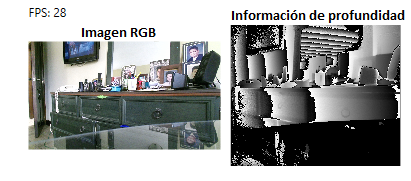
\includegraphics[]{graphics/RGB-D.PNG} \\
	\textbf{Fuente:} Tomado por el autor de tesis
\end{figure}  \\
La figura \ref{fig:RGBD}, fue capturado por el dispositivo, Kinect de XBox One, a una velocidad de 28 \acrfull{FPS}, cabe mencionar que los p�xeles  blancos de la imagen de la derecha, no se puede determinar el valor de profundidad, debido que falta el an�lisis de distancia, angulo relativo de la superficie, material de superficie, y otras variable m�s que se indicar� en el presente trabajo.
\subsubsection{Dispositivos en el mercado}
A continuaci�n se presentar� una lista de c�maras con sensor de profundidad, que se encuentra en el mercado hoy en d�a:
\begin{itemize}
	\item \textbf{ASUS XtionPro Live:} la corporaci�n ASUSTeK Computer \cite{xtionAsus}, desarroll� una c�mara con sensor de profundidad e infrarrojo, que permite detectar profundidad adaptativa, imagen en color y flujo de audio. Estas caracter�sticas permite capturar la imagen, el movimiento y la voz en tiempo real de un usuario. 
	\item \textbf{Structure Sensor:} La empresa, Occipital inc \cite{structureOccipital}, implementa un sensor de estructura, que permite escanear personas, espacios, mapas y objetos en 3D. 
	\item \textbf{Intel RealSense cameras:} Seg�n la tecnolog�a Intel RealSense \cite{intelRealSense}, permite detectar una alta velocidad de cuadros (p�xeles), RGB de calidad y la mejor resoluci�n de profundidad, en soluciones de realidad virtual, realidad aumentada, rob�tica, drones y otras aplicaciones m�s..
	\item \textbf{Microsoft Kinect:} Seg�n el estudio, Microsoft Kinect Sensor and its effect	\cite{zhang2012microsoft}, menciona que el Kinect contiene un sensor de profundidad, una c�mara a color y una matriz de micr�fonos que permite capturar movimientos, reconocer caracter�sticas faciales, construir un modelo del cuerpo en 3D y reconocer sonidos.
\end{itemize}
Tal como se observa en el listado, todas las c�maras de RGB-D permite detectar caracter�sticas del ambiente, por lo cual a la hora de escoger una c�mara se debe tomar en cuenta las siguientes especificaciones:
\begin{itemize}
	\item \textbf{Alcance del sensor 3D:} Seg�n el art�culo cient�fico, Kinect depth sensor evaluation for computer vision applications \cite{andersen2012kinect}, menciona que el alcance del sensor 3D es la medida m�xima de profundidad (z) desde un objeto hasta el sensor de profundidad.
	\item \textbf{3D Resoluci�n:} Hace referencia a la cantidad de p�xeles de la imagen que se obtiene del sensor de \gls{infrarrojo}.
	\item \textbf{RGB Resoluci�n:} Hace referencia a la cantidad de p�xeles de colores de una imagen.
	\item \textbf{\acrfull{FOV}:} Hace referencia al �ngulo m�ximo que puede detectar la c�mara, respecto a la horizontal(x) y la vertical (y).
	\item \textbf{Conexi�n:} Hace referencia al puerto de entrada y salida de la c�mara.
\end{itemize}
A continuaci�n se presentar� una comparaci�n de especificaciones entre las c�maras de RGB-D, mencionadas anteriormente:
\begin{table}[H]
\begin{center}
\caption{Comparaci�n de especificaciones entre c�maras de RGB-D }
\label{tab:RGBD}
\begin{tabular}{|l|l|l|l|l|l|} 
\hline
\textbf{Caracter�sticas}                                                          & \begin{tabular}[c]{@{}l@{}}\textbf{ASUS}\\\textbf{XtionPro}\\\textbf{Live}\end{tabular}   & \begin{tabular}[c]{@{}l@{}}\textbf{Structure}\\\textbf{Sensor}\end{tabular}  & \begin{tabular}[c]{@{}l@{}}\textbf{Intel}\\\textbf{RealSense}\\\textbf{SR300}\end{tabular}  & \begin{tabular}[c]{@{}l@{}}\textbf{Microsoft}\\\textbf{Kinect}\\\textbf{Live}\end{tabular} & \begin{tabular}[c]{@{}l@{}}\textbf{Microsoft}\\\textbf{Kinect}\\\textbf{v2}\end{tabular}	  \\ 
\hline
\begin{tabular}[c]{@{}l@{}}\textbf{Alcance del}\\\textbf{ sensor 3D}\end{tabular} & 0.8 a 3.5 m                                                                               & 0.4 a 3.5m                                                                   & 0.2 a 1.5m                                                                                  & 1.8 a 3.5m                                                                                 & 1.3 a 3.5m                                                                                  \\ 
\hline
\textbf{3D Resoluci�n}                                                            &\begin{tabular}[c]{@{}l@{}}640x480\\30fps\end{tabular}                   & \begin{tabular}[c]{@{}l@{}}640x480\\30fps\end{tabular}     & \begin{tabular}[c]{@{}l@{}}640x480\\60fps\end{tabular}                    &\begin{tabular}[c]{@{}l@{}}320x240\\30fps\end{tabular}					& \begin{tabular}[c]{@{}l@{}}512x424\\30fps\end{tabular}                    \\ 
\hline
\begin{tabular}[c]{@{}l@{}}\textbf{RGB}\\\textbf{ Resoluci�n}\end{tabular}        &\begin{tabular}[c]{@{}l@{}}1280x1024\\30fps\end{tabular}                   & \begin{tabular}[c]{@{}l@{}}640x480\\30fps\end{tabular}     & \begin{tabular}[c]{@{}l@{}}1920x1080\\30fps\end{tabular}                    &\begin{tabular}[c]{@{}l@{}}640x480\\30fps\end{tabular}					& \begin{tabular}[c]{@{}l@{}}1920x1080\\30fps\end{tabular}                    \\ 
\hline
\textbf{FOV}                                                                      & 58�H, 45�V                                                                                & 58�H, 45�V                                                                   & 73�H, 59�V                                                                                  & 57�H, 43�V                                                                                 & 70�H, 60�V                                                                                  \\ 
\hline
\textbf{Conexi�n}                                                                 & USB 2.0                                                                                   & USB 2.0                                                                      & USB 3.0                                                                                     & USB 2.0                                                                                    & USB 3.0                                                                                     \\
\hline
\end{tabular}
\end{center}
\textbf{Fuente:} Desarrollo de una aplicaci�n interactiva con Intel RealSense \cite{molero2018desarrollo} y Evaluation of the spatial resolution accuracy of the face tracking system for kinect for windows v1 and v2 \cite{amon2014evaluation}
\end{table}
En la tabla \ref{tab:RGBD}, se puede determinar que la c�maras, Intel RealSense SR300 y Microsoft Kinect V2, destacan de las dem�s c�maras debido  que tiene una mayor resoluci�n del sensor RGB y un campo de visi�n m�s amplio, por lo cual para el presente proyecto se seleccionar� la c�mara Microsoft Kinect V2. 